\subsubsection{PCM}
$PCM$ is a cluster of shared memory machines, thus all considerations reguarding mapping of processes to cores made in~\ref{fram-intr} become matter of study. Even the official guide of \textit{mvapich2}, the version of MPI that we have used to exploit Infiniband, emphasizes the importance of process-to-core mapping: as shown in~\cite{MVAPICH2-MAPPING}, different allocations of processes to cores can have a significant impact on the cost of communications. In principle, an entire study could be dedicated to this topic, leading to a lot of possible mappings, each one based on its reasonable heuristic. Obviously, we had to limit our analysis to a subset of the most simple mappings. In particular, we have studied the following configurations:   
\begin{itemize}
\item \textbf{Sequential mapping}. Adjacent ranks mapped on adjacent \textit{cores}. E.g., given two CPUs each one with 4 cores and 8 MPI processes, rank 0 goes on the first core of the \textit{first} CPU, rank 1 goes on the second core of the \textit{first} CPU, ..., rank 5 goes on the first core of the \textit{second} CPU and so on.
\item \textbf{Interleaved mapping}. Adjacent ranks mapped on adjacent \textit{CPUs}. E.g., given two CPUs each one with 4 cores and 8 MPI processes, rank 0 goes on the first core of the \textit{first} CPU, rank 1 goes on the first core of the \textit{second} CPU, rank 2 goes on the second core of the \textit{first} CPU and so on.
\item \textbf{Algorithm-specific mapping}. We have also studied a few mapping based on the nature of a specific Sorting Algorithm, like \textit{Mergesort} and \textit{Quicksort}. For instance, a mapping could be designed to let the most critical part of a stencil to take place in shared memory rather than inter-node.  
\end{itemize}
In the following, we will consider only the \textit{sequential mapping} because we have practically experienced that collective communications (in particular, the \textit{gather}) are more cost-effective than for other mappings. For more informations about the results obtained with other mappings the reader could refer to specific material attached to this report.


\paragraph{Scalability of Sorting Algorithms}

\begin{figure}[t]
	\begin{center}
		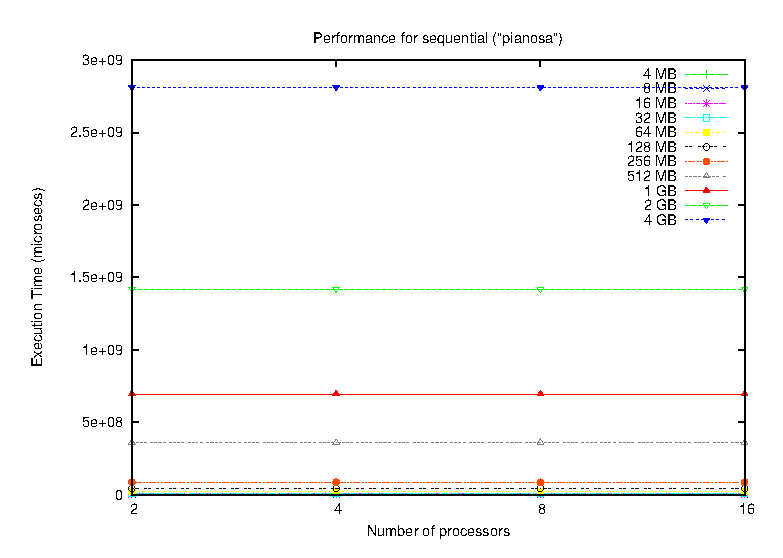
\includegraphics[scale=0.6]{plots/test_01_pianosa/NxTxM/sequential_pianosa_NxTxM}
	\end{center}
  	\caption{\textit{PCM}. Completion Time for the Sequentialsort.}
  	\label{sequential-PCM}
\end{figure}

\begin{figure}[h]
	\centering
	\subfloat[Quicksort.]{\label{NxTxM-sequential}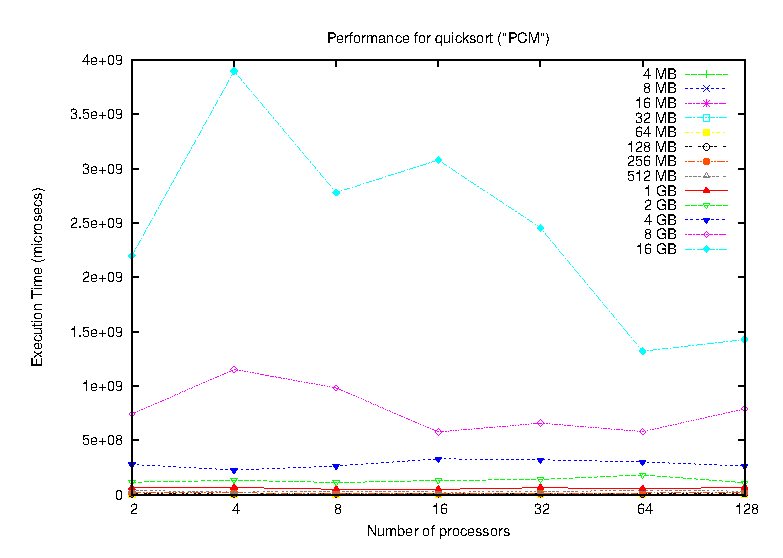
\includegraphics[width=0.4\textwidth]{plots/test_01_PCM/NxTxM/quicksort_PCM_NxTxM}} 
	\hspace*{20pt}	
  	\subfloat[Bitonicsort.]{\label{NxTxM-bitonicsort}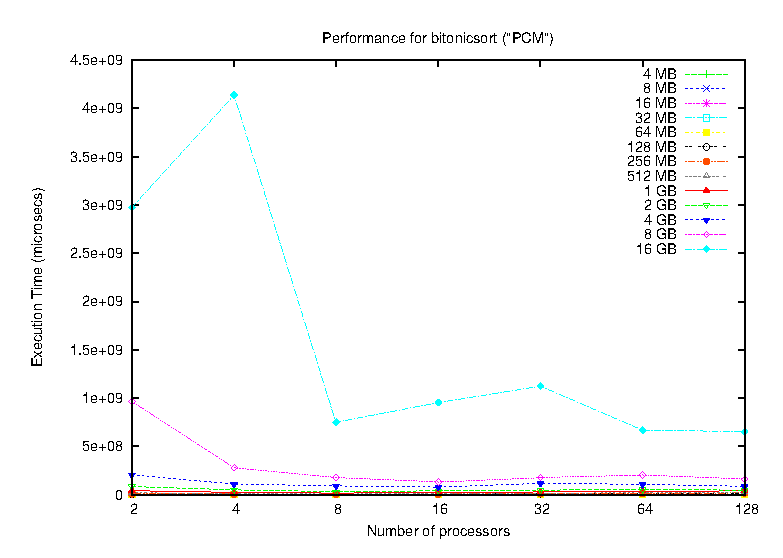
\includegraphics[width=0.4\textwidth]{plots/test_01_PCM/NxTxM/bitonicsort_PCM_NxTxM}} 
	
	\centering
	\subfloat[Bucketsort.]{\label{NxTxM-bucketsort}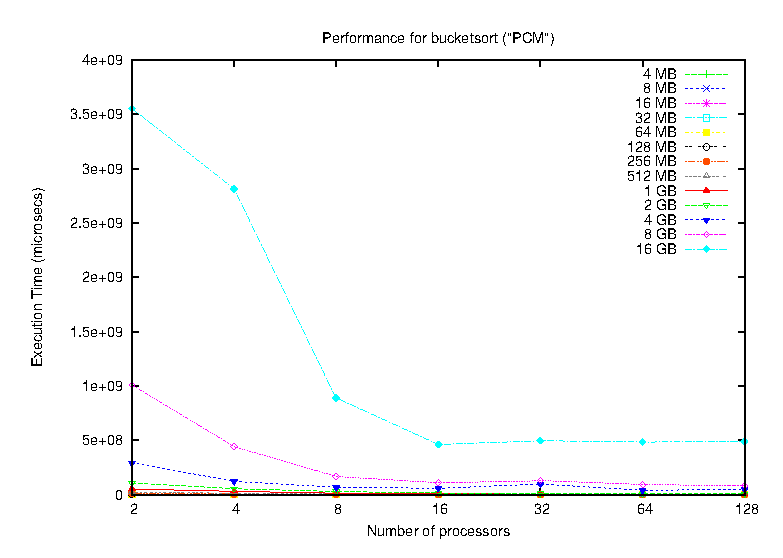
\includegraphics[width=0.4\textwidth]{plots/test_01_PCM/NxTxM/bucketsort_PCM_NxTxM}} 
  	\hspace*{20pt}
  	\subfloat[Samplesort.]{\label{NxTxM-samplesort}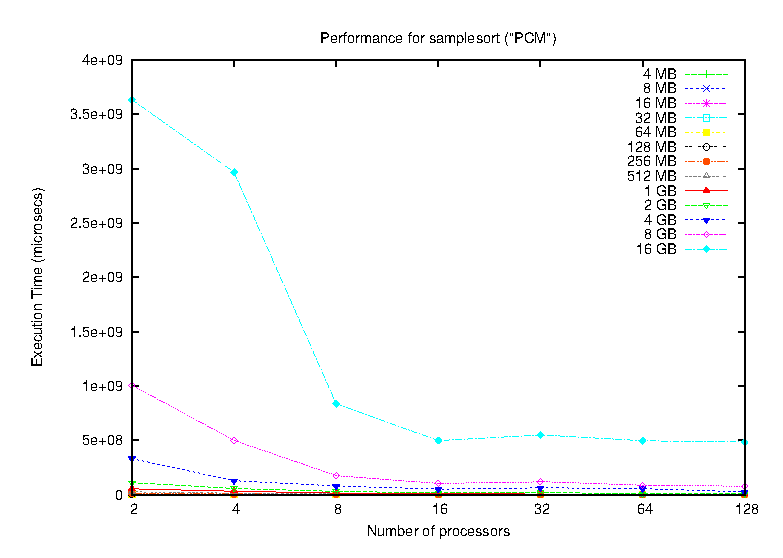
\includegraphics[width=0.4\textwidth]{plots/test_01_PCM/NxTxM/samplesort_PCM_NxTxM}} 
	
	\centering
  	\subfloat[Mergesort.]{\label{NxTxM-mergesort}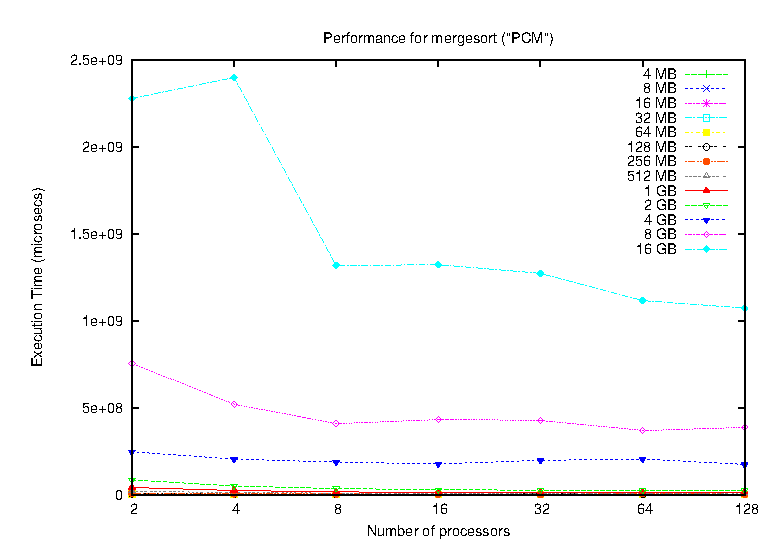
\includegraphics[width=0.4\textwidth]{plots/test_01_PCM/NxTxM/mergesort_PCM_NxTxM}}   
  	\hspace*{20pt}  
  	\subfloat[4-Way Mergesort.]{\label{NxTxM-kmerge}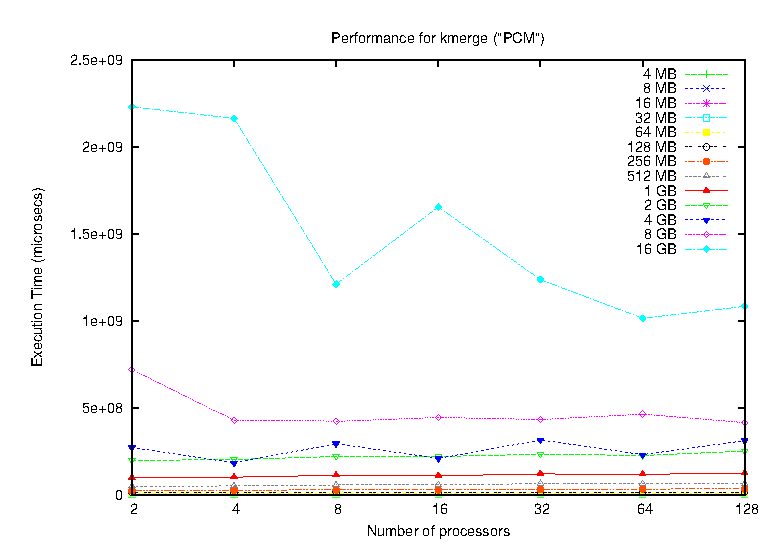
\includegraphics[width=0.4\textwidth]{plots/test_01_PCM/NxTxM/kmerge_PCM_NxTxM}} 
	
	\centering
  	\subfloat[Load-Balanced Mergesort.]{\label{NxTxM-lbmergesort}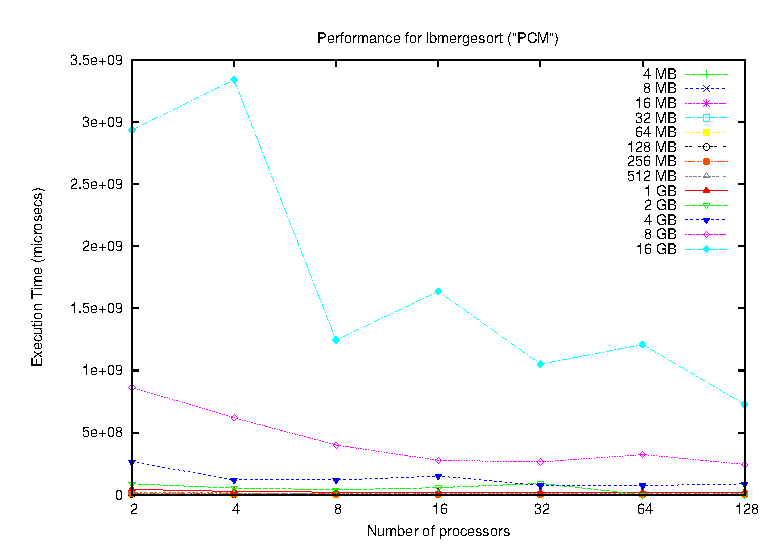
\includegraphics[width=0.4\textwidth]{plots/test_01_PCM/NxTxM/lbmergesort_PCM_NxTxM}} 
  	\hspace*{20pt}  
  	\subfloat[Load-Balanced Multi-Way Mergesort.]{\label{NxTxM-lbkmergesort}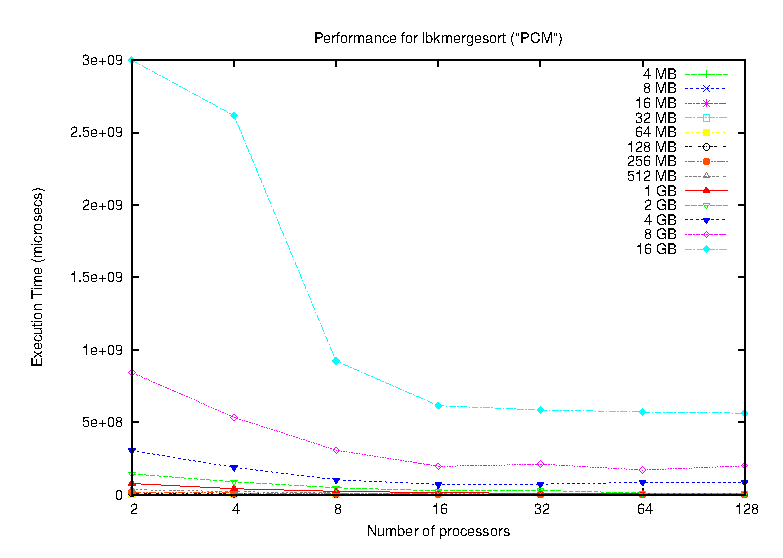
\includegraphics[width=0.4\textwidth]{plots/test_01_PCM/NxTxM/lbkmergesort_PCM_NxTxM}} 	
  	
	\caption{\textit{PCM}. Time Completion of Sorting Algorithms by varying the parallelism degree. Each shape on a graphic represents the Time Completion of a certain Sorting Algorithm for a data set of specific size.}
	\label{NxTxM}
\end{figure}
 
\begin{figure}[!ht]
	\centering
	\subfloat[Quicksort.]{\label{MxTxN-sequential}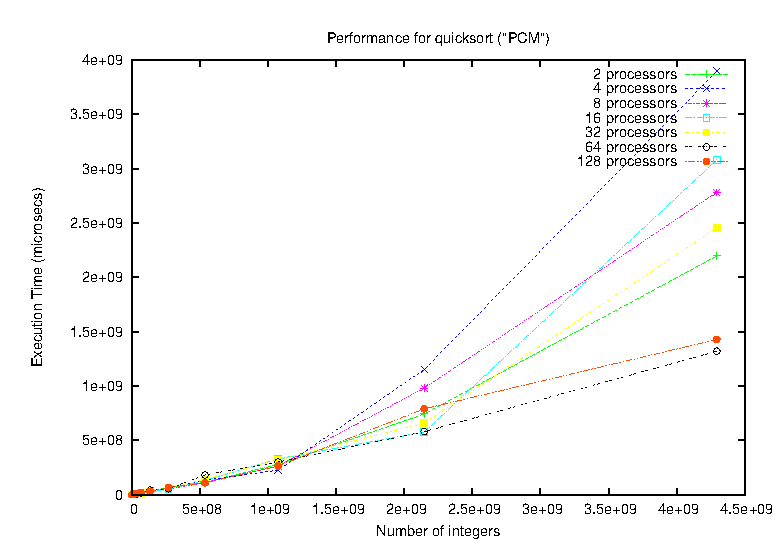
\includegraphics[width=0.4\textwidth]{plots/test_01_PCM/MxTxN/quicksort_PCM_MxTxN}} 
	\hspace*{20pt}	
  	\subfloat[Bitonicsort.]{\label{MxTxN-bitonicsort}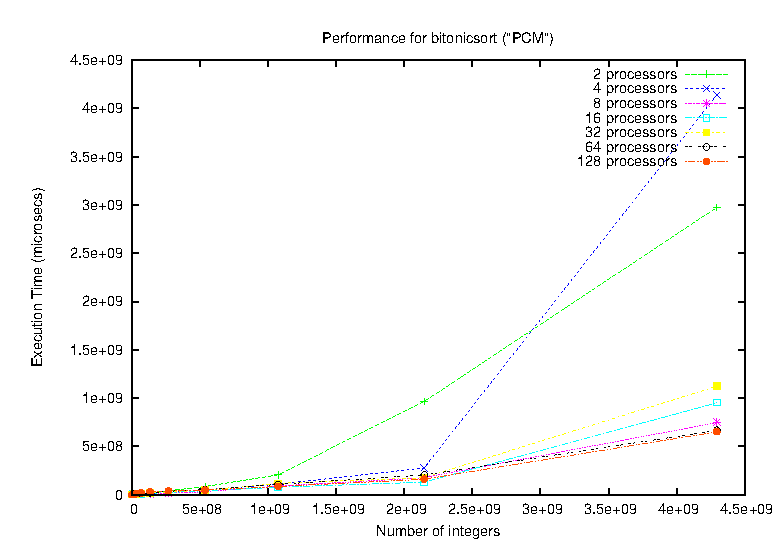
\includegraphics[width=0.4\textwidth]{plots/test_01_PCM/MxTxN/bitonicsort_PCM_MxTxN}} 
  		
	\centering
	\subfloat[Bucketsort.]{\label{MxTxN-bucketsort}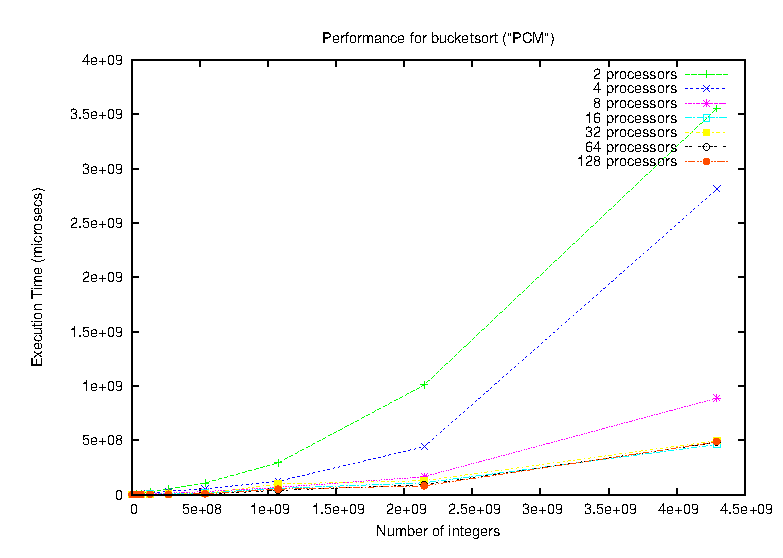
\includegraphics[width=0.4\textwidth]{plots/test_01_PCM/MxTxN/bucketsort_PCM_MxTxN}} 
  	\hspace*{20pt}
  	\subfloat[Samplesort.]{\label{MxTxN-samplesort}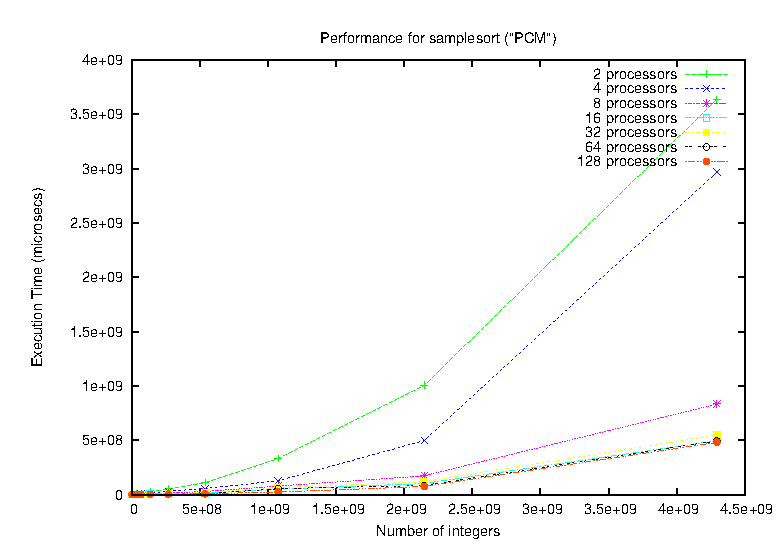
\includegraphics[width=0.4\textwidth]{plots/test_01_PCM/MxTxN/samplesort_PCM_MxTxN}} 
	
	\centering
  	\subfloat[Mergesort.]{\label{MxTxN-mergesort}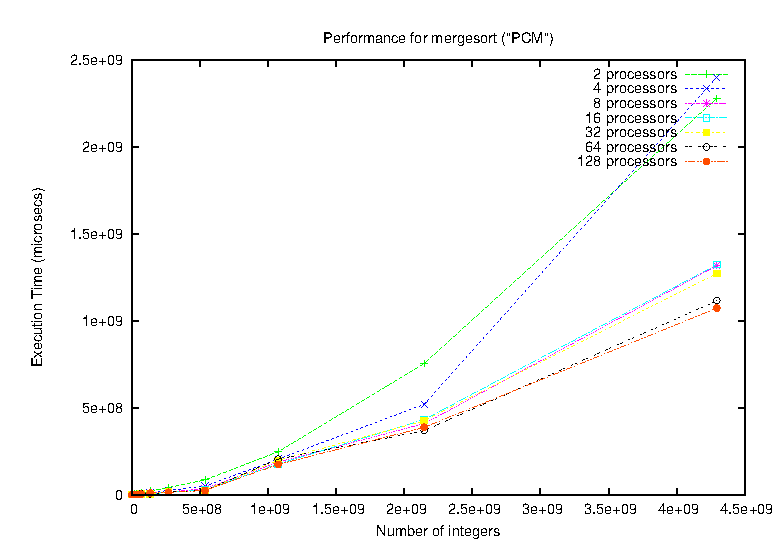
\includegraphics[width=0.4\textwidth]{plots/test_01_PCM/MxTxN/mergesort_PCM_MxTxN}}   
  	\hspace*{20pt}  
  	\subfloat[4-Way Mergesort.]{\label{MxTxN-kmerge}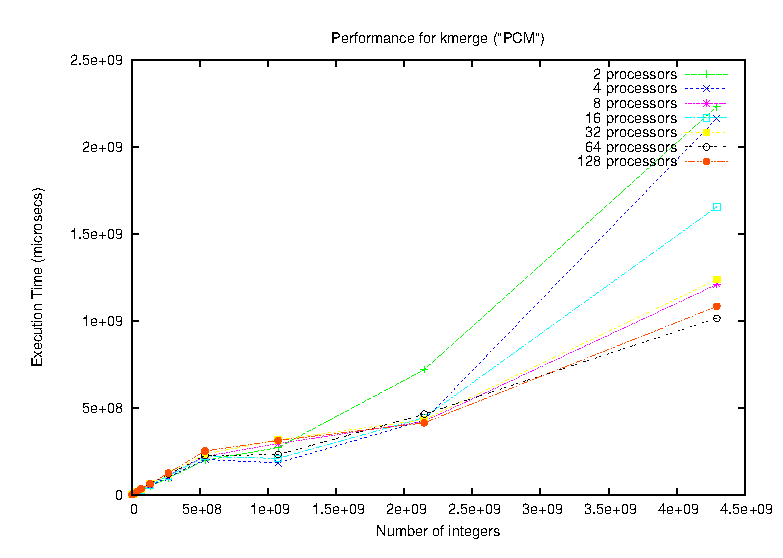
\includegraphics[width=0.4\textwidth]{plots/test_01_PCM/MxTxN/kmerge_PCM_MxTxN}} 
	
	\centering
  	\subfloat[Load-Balanced Mergesort.]{\label{MxTxN-lbmergesort}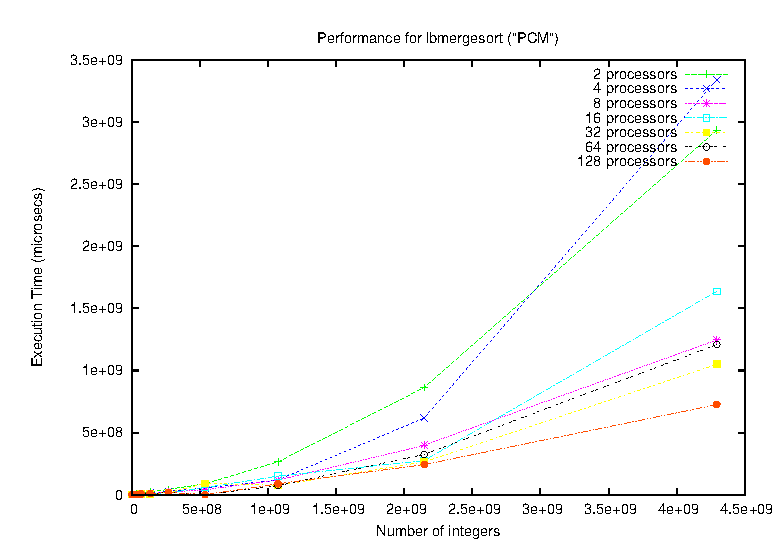
\includegraphics[width=0.4\textwidth]{plots/test_01_PCM/MxTxN/lbmergesort_PCM_MxTxN}} 
  	\hspace*{20pt}  
  	\subfloat[Load-Balanced Multi-Way Mergesort.]{\label{MxTxN-lbkmergesort}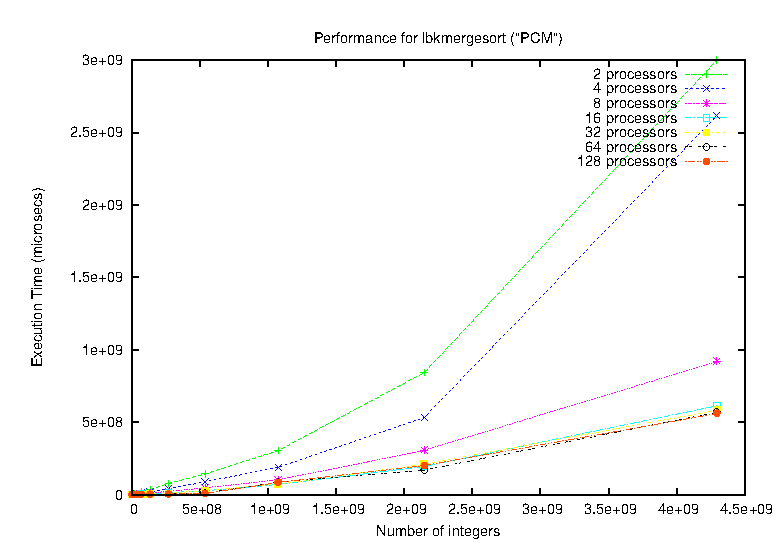
\includegraphics[width=0.4\textwidth]{plots/test_01_PCM/MxTxN/lbkmergesort_PCM_MxTxN}} 
  	
	\caption{\textit{PCM}. Time Completion of Sorting Algorithms for increasing sizes of the data set. }
	\label{MxTxN}
\end{figure} 
  
\paragraph{Comparison between Sorting Algorithms}


\begin{figure}[!ht]
	\centering
	\subfloat[Data set of 1M integers.]{\label{NxTxA-1M}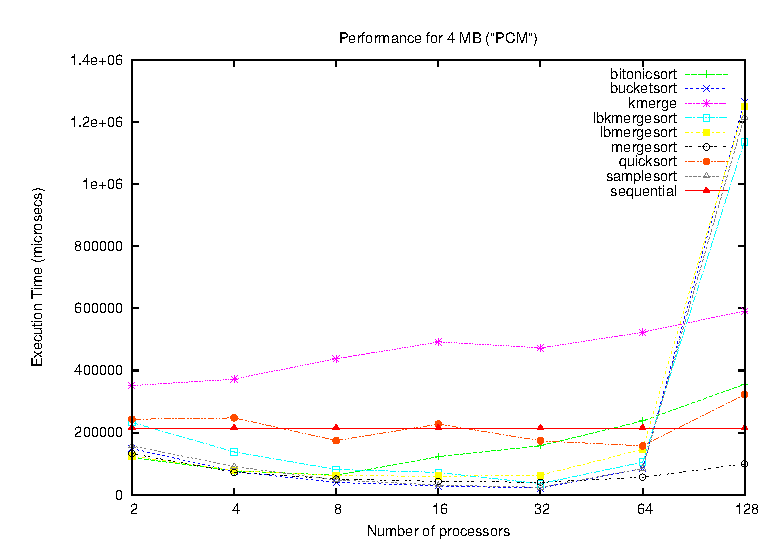
\includegraphics[width=0.4\textwidth]{plots/test_01_PCM/NxTxA/M1048576_PCM_NxTxA}} 
	\hspace*{20pt}	
  	\subfloat[Data set of 2M integers.]{\label{NxTxA-2M}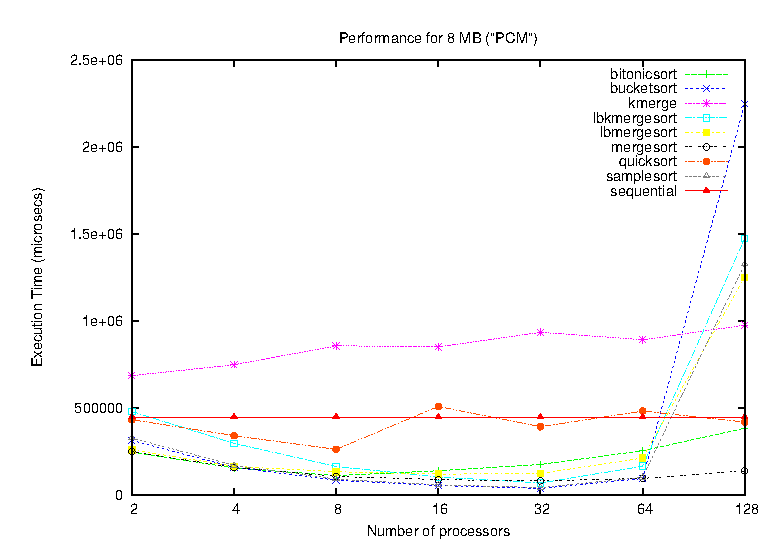
\includegraphics[width=0.4\textwidth]{plots/test_01_PCM/NxTxA/M2097152_PCM_NxTxA}} 
  		
	\centering
	\subfloat[Data set of 4M integers.]{\label{NxTxA-4M}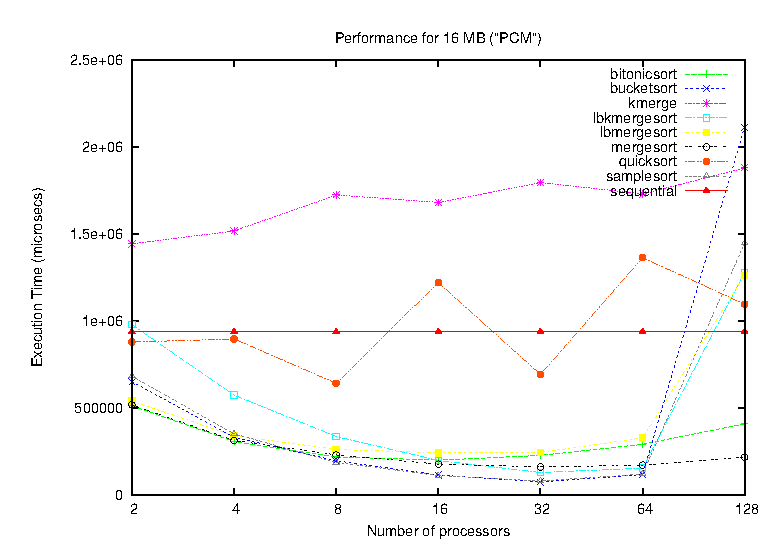
\includegraphics[width=0.4\textwidth]{plots/test_01_PCM/NxTxA/M4194304_PCM_NxTxA}} 
  	\hspace*{20pt}
  	\subfloat[Data set of 8M integers.]{\label{NxTxA-8M}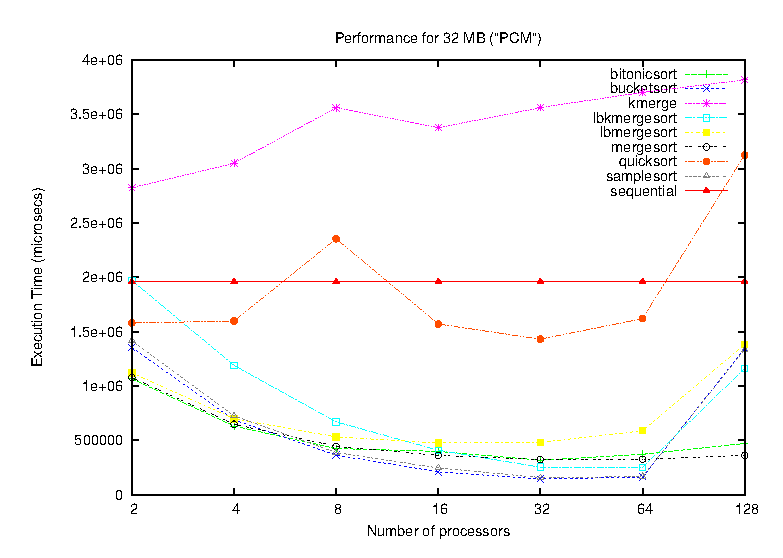
\includegraphics[width=0.4\textwidth]{plots/test_01_PCM/NxTxA/M8388608_PCM_NxTxA}} 
	
	\centering
  	\subfloat[Data set of 16M integers.]{\label{NxTxA-16M}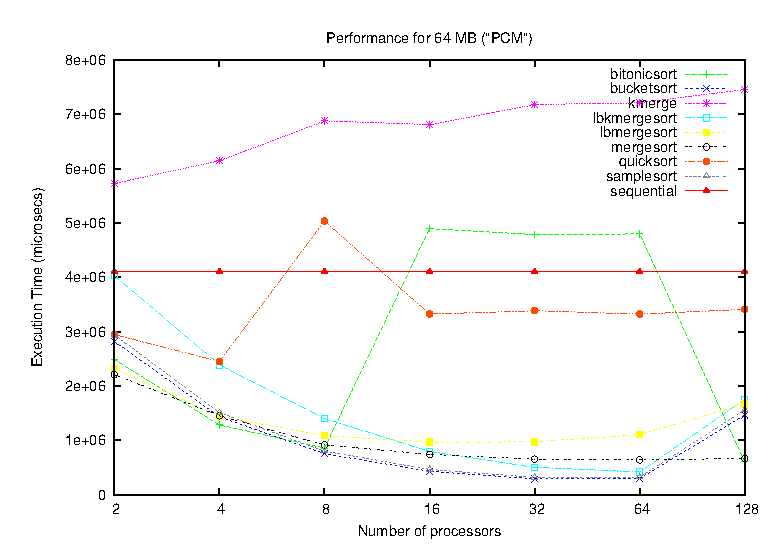
\includegraphics[width=0.4\textwidth]{plots/test_01_PCM/NxTxA/M16777216_PCM_NxTxA}}   
  	\hspace*{20pt}  
  	\subfloat[Data set of 32M integers.]{\label{NxTxA-32M}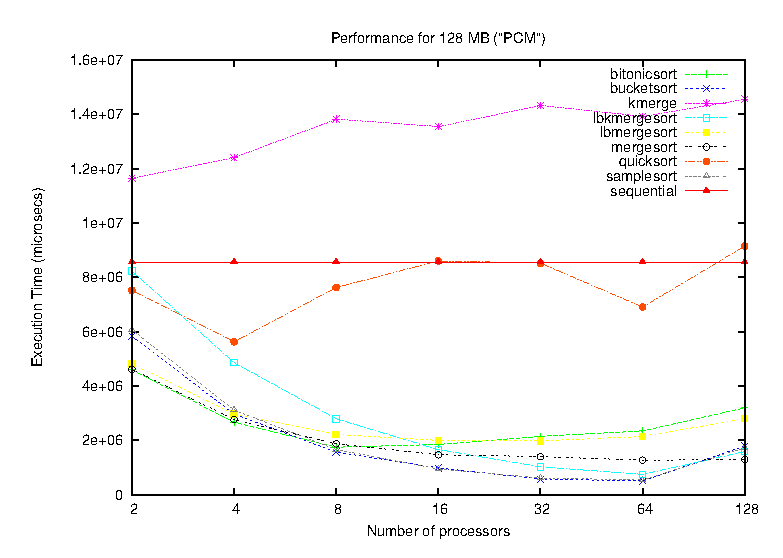
\includegraphics[width=0.4\textwidth]{plots/test_01_PCM/NxTxA/M33554432_PCM_NxTxA}} 
  	
	\caption{\textit{PCM}. Time Completion for sorting \textit{small} data sets. Each graphic represents a data set of fixed size, while each shape on a graphic shows the Time Completion of a certain Sorting Algorithm for that data set.}
	\label{NxTxA-small}
\end{figure} 

\begin{figure}[!ht]
	\centering
	\subfloat[Data set of 64M integers.]{\label{NxTxA-64M}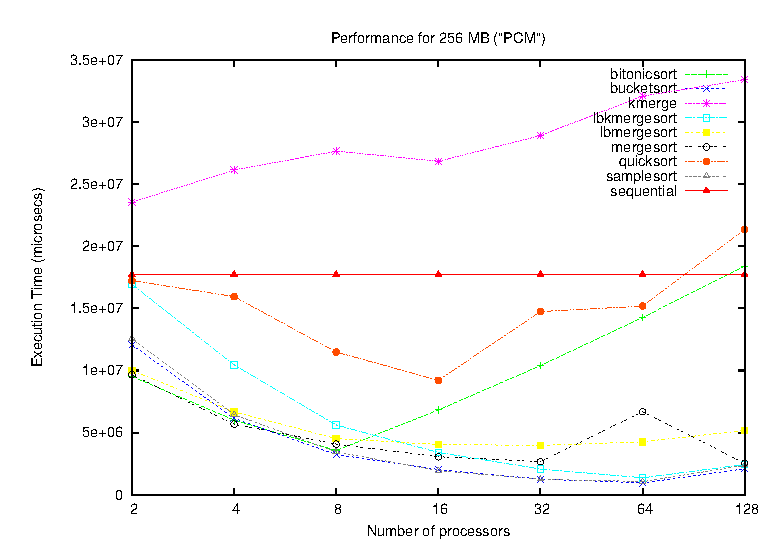
\includegraphics[width=0.5\textwidth]{plots/test_01_PCM/NxTxA/M67108864_PCM_NxTxA}} 
	
	\centering
  	\subfloat[Data set of 128M integers.]{\label{NxTxA-128M}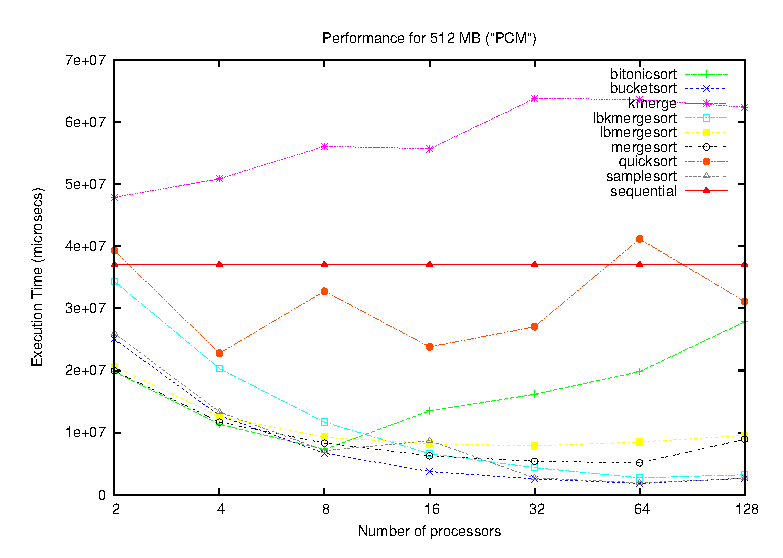
\includegraphics[width=0.5\textwidth]{plots/test_01_PCM/NxTxA/M134217728_PCM_NxTxA}} 
  		
	\centering
	\subfloat[Data set of 256M integers.]{\label{NxTxA-256M}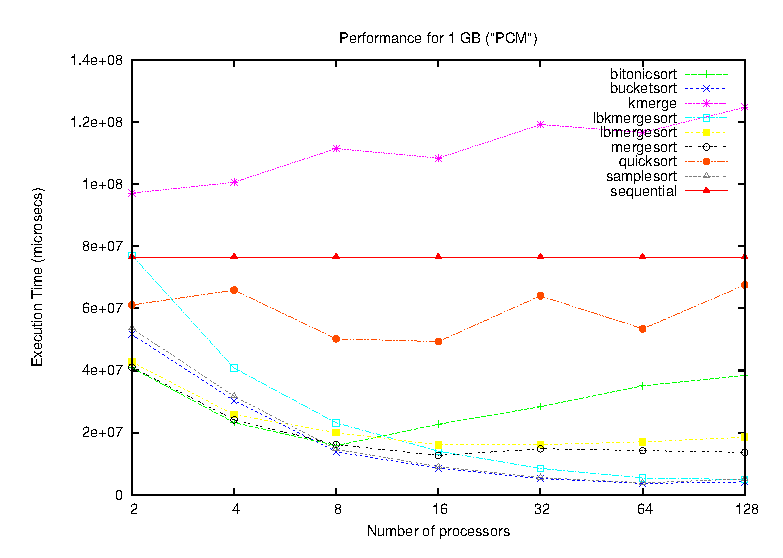
\includegraphics[width=0.5\textwidth]{plots/test_01_PCM/NxTxA/M268435456_PCM_NxTxA}} 
  	
  	\caption{\textit{PCM}. Time Completion for sorting \textit{large} data sets. Each graphic represents a data set of fixed size, while each shape on a graphic shows the Time Completion of a certain Sorting Algorithm for that data set.}
	\label{NxTxA-large}
\end{figure}

\begin{figure}[!ht]  	
  	\centering
  	\subfloat[Data set of 512M integers.]{\label{NxTxA-512M}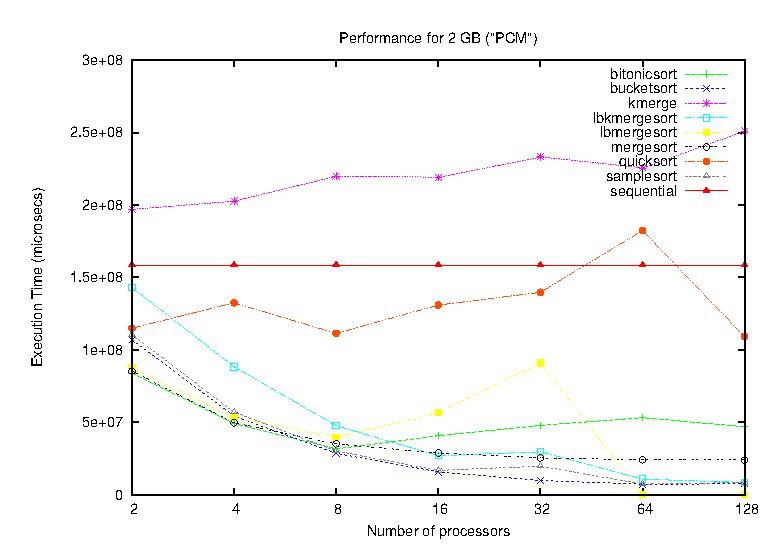
\includegraphics[width=0.4\textwidth]{plots/test_01_PCM/NxTxA/M536870912_PCM_NxTxA}} 
	\hspace*{20pt}  
  	\subfloat[Data set of 1G integers.]{\label{NxTxA-1G}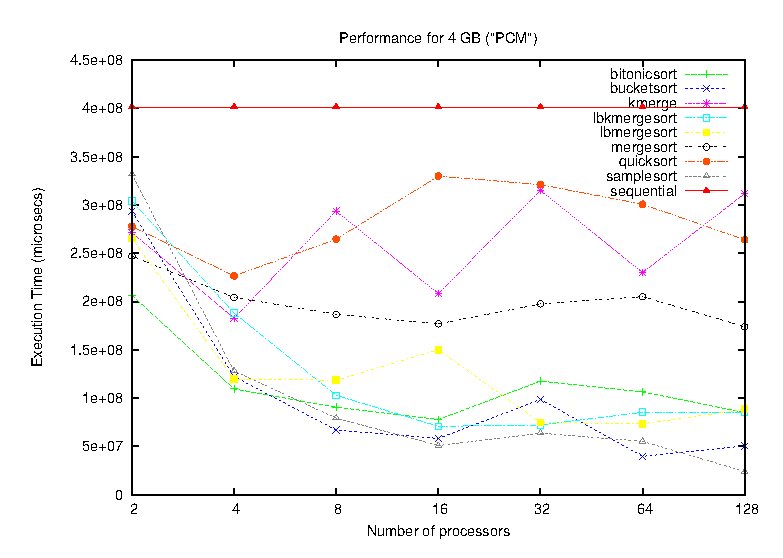
\includegraphics[width=0.4\textwidth]{plots/test_01_PCM/NxTxA/M1073741824_PCM_NxTxA}}   
	
	\centering
  	\subfloat[Data set of 2G integers.]{\label{NxTxA-2G}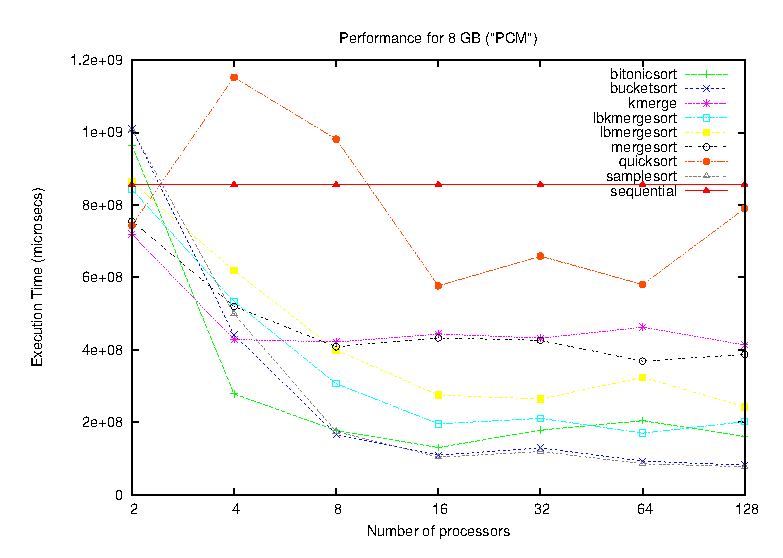
\includegraphics[width=0.4\textwidth]{plots/test_01_PCM/NxTxA/M2147483648_PCM_NxTxA}}  
	\hspace*{20pt}  
  	\subfloat[Data set of 4G integers.]{\label{NxTxA-4G}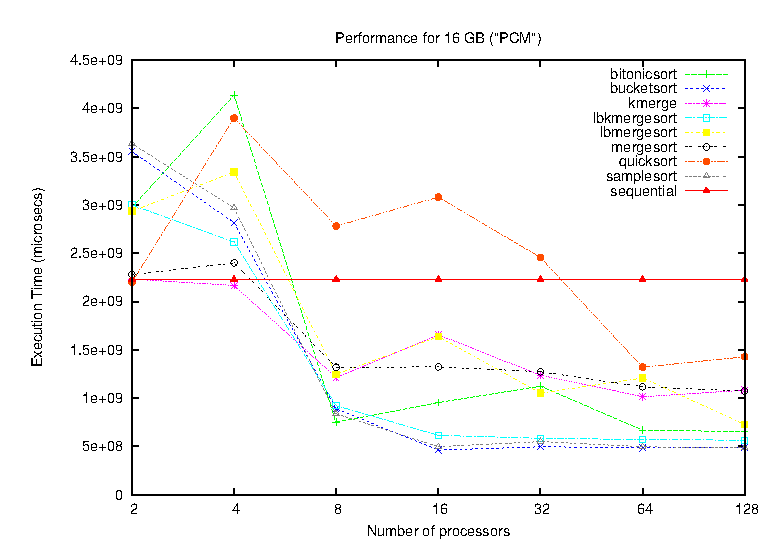
\includegraphics[width=0.4\textwidth]{plots/test_01_PCM/NxTxA/M4294967296_PCM_NxTxA}}   
  	
	\caption{\textit{PCM}. Time Completion for sorting \textit{huge} data sets. Each graphic represents a data set of fixed size, while each shape on a graphic shows the Time Completion of a certain Sorting Algorithm for that data set.}
	\label{NxTxA-huge}
\end{figure} 

\begin{figure}[!ht]
	\centering
	\subfloat[Parallelism degree 2.]{\label{MxTxA-n2}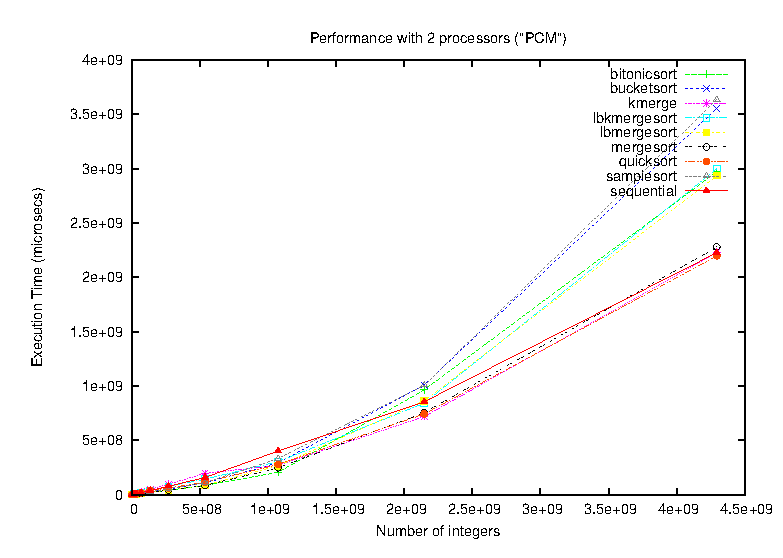
\includegraphics[width=0.4\textwidth]{plots/test_01_PCM/MxTxA/n2_PCM_MxTxA}} 
	\hspace*{20pt}	
  	\subfloat[Parallelism degree 4.]{\label{MxTxA-n4}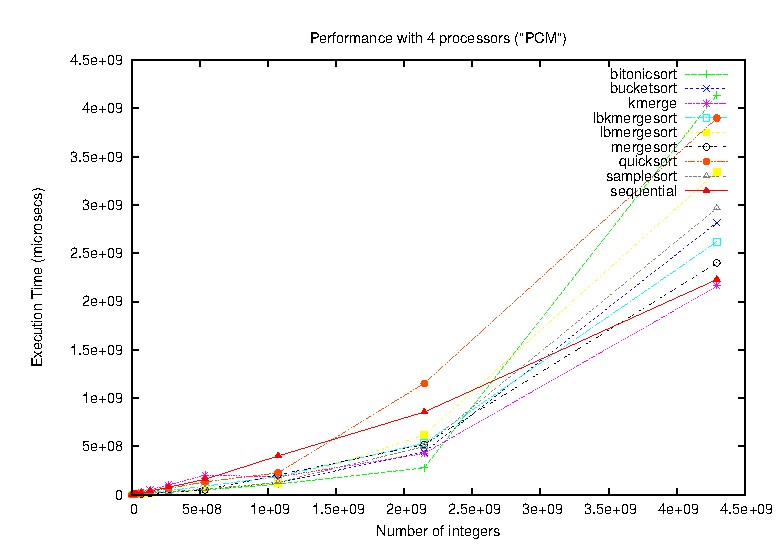
\includegraphics[width=0.4\textwidth]{plots/test_01_PCM/MxTxA/n4_PCM_MxTxA}} 
  		
	\centering
	\subfloat[Parallelism degree 8.]{\label{MxTxA-n8}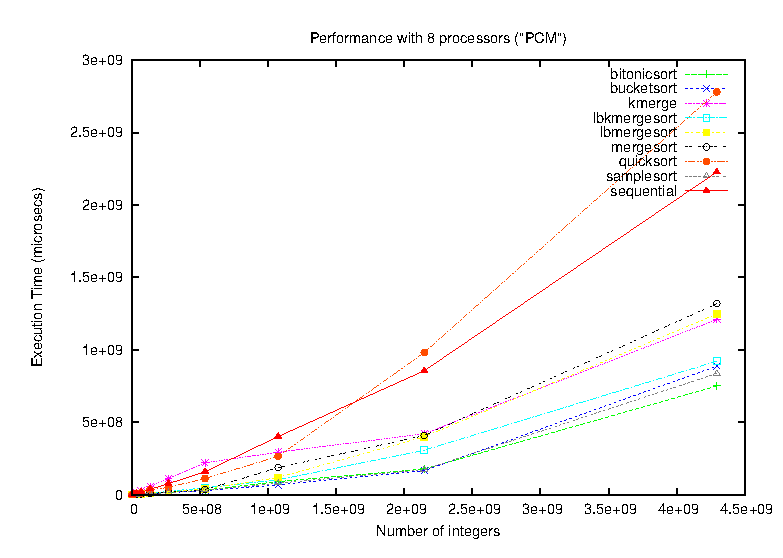
\includegraphics[width=0.4\textwidth]{plots/test_01_PCM/MxTxA/n8_PCM_MxTxA}} 
  	\hspace*{20pt}
  	\subfloat[Parallelism degree 16.]{\label{MxTxA-n16}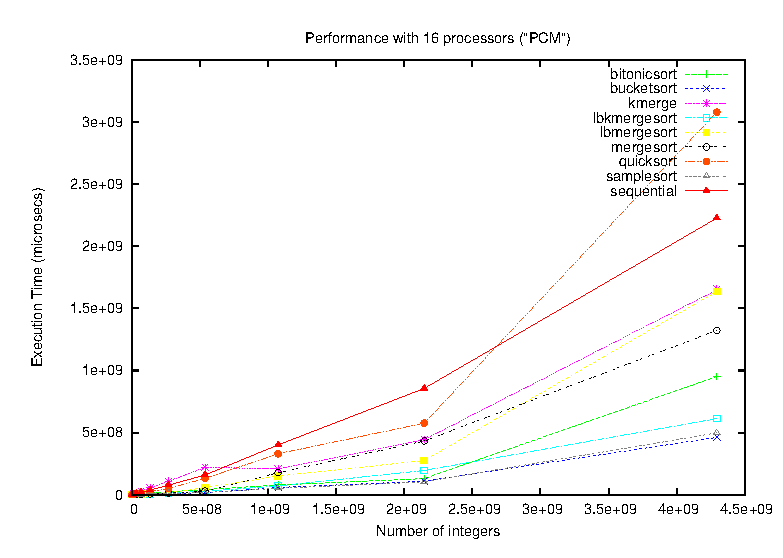
\includegraphics[width=0.4\textwidth]{plots/test_01_PCM/MxTxA/n16_PCM_MxTxA}} 
  		
	\centering
	\subfloat[Parallelism degree 32.]{\label{MxTxA-n32}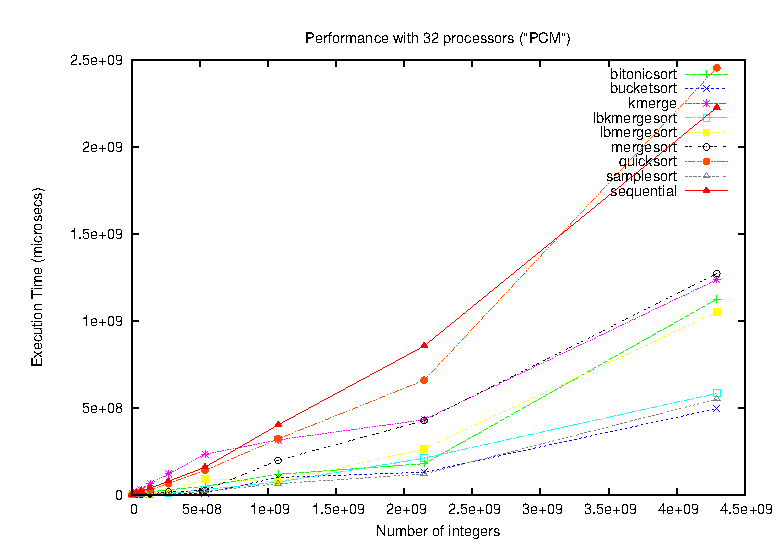
\includegraphics[width=0.4\textwidth]{plots/test_01_PCM/MxTxA/n32_PCM_MxTxA}} 
  	\hspace*{20pt}
  	\subfloat[Parallelism degree 64.]{\label{MxTxA-n64}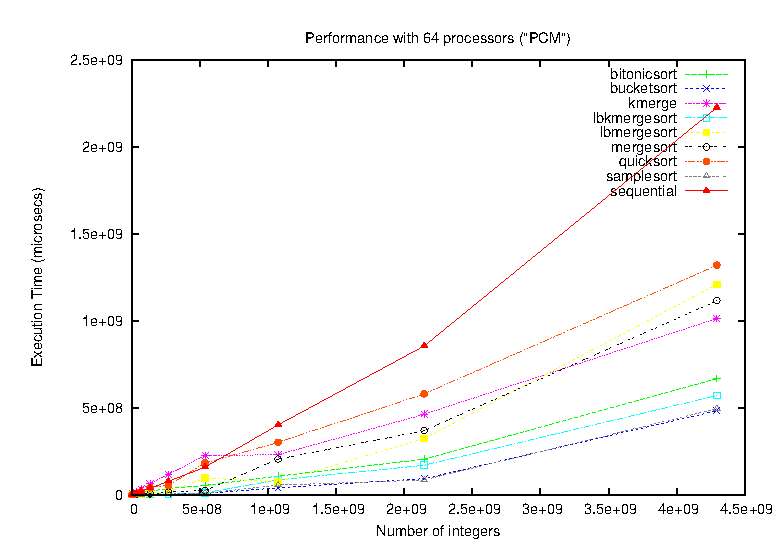
\includegraphics[width=0.4\textwidth]{plots/test_01_PCM/MxTxA/n64_PCM_MxTxA}} 
  	
	\centering
	\subfloat[Parallelism degree 128.]{\label{MxTxA-n128}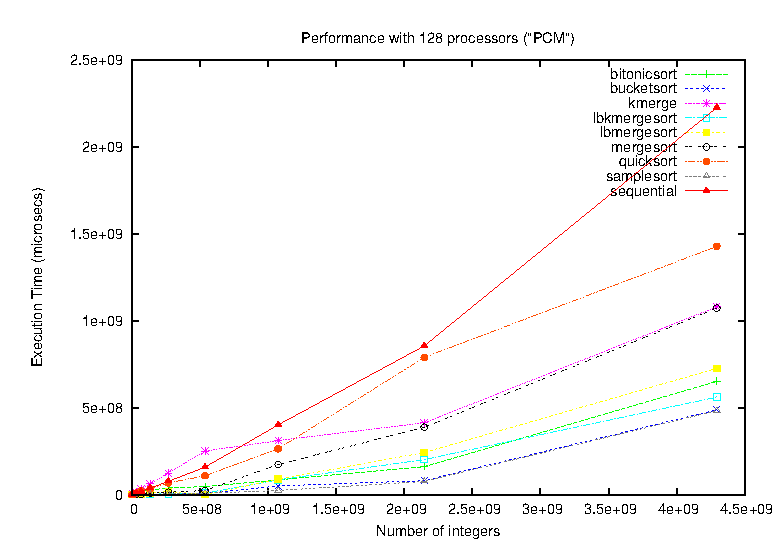
\includegraphics[width=0.4\textwidth]{plots/test_01_PCM/MxTxA/n128_PCM_MxTxA}} 
  	
	\caption{\textit{PCM}. Time Completion for sorting data sets with fixed parallelism degree.}
	\label{MxTxA}
\end{figure} 

\clearpage